\documentclass[hidelinks, 12pt, oneside]{article}
\usepackage{bookmark}
\usepackage{graphicx}
\usepackage{hyperref}
\graphicspath{{images/}}
\usepackage[utf8]{inputenc}
\usepackage[english]{babel}

\begin{document}
 
%titlepage
\thispagestyle{empty}
\begin{center}
\begin{minipage}{0.75\linewidth}
    \centering
    
%University logo
    
\includegraphics{UPlogo}
    \rule{0\linewidth}{0.15\linewidth}\par

%Thesis title
    {\uppercase{\Large COS 301 Mini Project\par}}
   	{\Large Top Level Integration Testing \par} 
    \vspace{1cm}
%Author's name
    {\normalsize Elana Kuun u12029522\par}
    {\normalsize Hlavutelo Maluleke u12318109\par}
    {\normalsize Estian Rosslee u12223426\par}
    {\normalsize David Breetzke u12056503\par}
    {\normalsize Sylvester Mpungane u11241617\par}
    {\normalsize Phethile Mkhabela u12097561\par}
    {\normalsize Renaldo van Dyk  u12204359\par}
    {\normalsize Antonia Michael  u13014171\par}
    {\normalsize Herman Keuris  u13037618\par}
    {\normalsize Jaco-Louis Kruger  u13025105\par}
    \vspace{1cm}
    
    \href{https://github.com/Jaco-Louis/Top-level-testing.git}{Github Repository}\par
    \vspace{1cm}
%Date
    {\Large April 2015}
\end{minipage}
\end{center}
\clearpage

\tableofcontents

\newpage

\section{Introduction}
This document contains the findings of the various activities performed as per testing of the Buzz Space system top level integration.

\section{Testing Results}
\subsection{Top Level A Testing Results}
\subsubsection{Functional Testing}
\subsubsection{Non-functional Testing} 

\begin{enumerate}
\item Usability:

The system is usable because firstly the necessary actions that a user can take appear in a navigation bar at the top of the screen. Thus it is easy for a novice user to be able to know what to click on and navigate the website. 

The interface is not cluttered, and only basic functionality is displayed on the home screen, making the system more learnable. The buttons are labelled with text rather than with graphical icons, and the text on the button is quite explanatory, which makes their purpose more clear. 

Larger headings are used to label the different sections, for example under the Manage Constraints tab there are large headings to indicate the Existing constraints section and the Add new constraint section. This again contributes to ease of use for the novice first year user.

Through these mechanisms the system is memborable hence it is also be understandable.  

\item Integratibility:

The system is able to address future integration requirements by providing access to its services using widely adopted public standards such as firstly having separate npm packages for all the different modules. The packages are stored on Synopia. Also, electrolyte is being used in the server to provide a dependency injection. The HandleBars server is the main server that needs to be used to test and integrate all the modules on. The routes/index.js, routes/infrastructure.js and routes/content.js files use express to route the different hbs files for the different modules in order to integrate the infrastructure and content subsystems into the main system. 

A separate file is used to establish the connection to the database to avoid having this done in all the separate files. Also, global variables are now used such as the global password and username for example. 

A document has been provided via email and a README file has been provided to specify important standards and regulations that must be followed.

The functional code in the separate packages must be placed in an exportable function taking parameters such as the database or settings, and this is done as part of the electrolyte dependency injection. 

Exports are also used in the different files to make the code accessible to the other files.

\item Deployability:

The system is deployable on Linux servers as we have run it using Ubuntu 14.04 Linux and the system was able to run. The following screenshot shows the system running on a Linux server:

The system is deployable on an environment using different databases for persistence of the Buzz database because the Handlebars server contains a folder called node\_modules, and it contains the buzz\_database package. This package can easily be swapped out and an alternative database package can be plugged in, that the system can use due to the flexibility of this server. As long as the new package has the same name so that the files that require the database do not need to be changed, no major changes will need to be made.  
//screenshot

The system is deployable in environments where the user authentication credentials and roles are sourced from different repositories. The following screenshot indicates that the Handlebars server contains a folder called node\_modules, and it contains the buzz\_csds package. 
//screenshot

This package can easily be swapped out and an alternative data source package with different credentials and roles can be used, due to the pluggability of the system and dependency injection employed by the top level team. The new package must just be named the same as the old one to avoid errors where the file is required from the package in the code. 

\end{enumerate}


\subsection{Top Level B Testing Results}

\subsubsection{Functional Testing}

\begin{enumerate}
\item Buzz Resources Module

\textbf{Description}
	
The system suppose to integrate a resource module that is used to upload and manage resources like media files and documents that can either linked or embedded to a post.
	
\textbf{Preconditions}
\begin{itemize}
	\item Size constraints must be met
	\item The resource mimetype must be detected
	\item The resource to must be supported
\end{itemize}

\textbf{Post-conditions}
\begin{itemize}
\item Url for resource must be generated
\item Resource must persist
\end{itemize}

\textbf{Test Results}

The Buzz resources module works when test in isolation through unit testing but fails on automated integration testing, it was not integrated as required by system specification. 



		 		 
\item Buzz Notification Module

\textbf{Description}

This module is focused on registering for notification messages, for submitted threads and the posting of a particular user and any possible notification that one can receive for their posts via email.
 	
\textbf{Preconditions}
\begin{itemize}
	\item User must have registered to receive notifications 
\end{itemize}

\textbf{Post-conditions}
\begin{itemize}
\item User should receive all notification based on the domain (received from all threads or a particular thread) the user registered for to receive notifications.   
\end{itemize}

\textbf{Test Results}

The Buzz notification was not integrated for this system, no email notifications are sent when a thread or post is submitted. 
\item Buzz-Status module
	
The Buzz-Status module was expected to at least implement these 6 functional processes:
	
\begin{enumerate}
	\item assessProfile:
	\begin{itemize}
		\item\textbf{Objective: } Serve as a general interface through which lecturers can choose a pluggable implementation with which to assess user profiles.
		\item\textbf{Pre-conditions: } Have some form of administrative users and general users. It should also have profiles for users of the Buzz system. 
		\item\textbf{Post-conditions: } ProfileAssessor can return the queried information about a the profile of a user, according to various criteria but iy should, as a minimal requirement, at least be able to calculate the user’s status (i.e. the user’s rating).
		\item\textbf{Testing: } Although both pre-conditions were met, no actual implementation for this functional requirement is present in the Buzz system (meaning post-conditions were not met).
	\end{itemize}
\item setStatusCalculator:
	\begin{itemize}
		\item\textbf{Objective: } An interface through which a StatusCalculator can be assigned. The StatusCalculator is used to assign a status value to a user according to specific criteria. The default StatusCalculator should be NumPostAssesor which assigns a status directly proportional to the number of posts a user has made.
		\item\textbf{Pre-conditions: } It should have some form of administrative and general users. It should have profiles for users of the Buzz system. It should have a space where users can post content (this is a pre-condition for the default StatusCalculator, i.e. NumPostAssessor).
		\item\textbf{Post-conditions: } The assigned StatusCalculator must be able to assign a status value to all users.
		\item\textbf{Testing: } Only the first two pre-conditions are met. Although there is a space where users can post content (i.e. http://buzz-codechat.rhcloud.com/spaces/) it does not fulfil any of its required functionality (i.e. can’t successfully post content, no thread handling). There is no implementation of a StatusCalculator present in the Buzz system, therefore no post-conditions were met.
	\end{itemize}
\item getStatusForProfile:
	\begin{itemize}
		\item\textbf{Objective: } A simple query which returns the user’s status.
		\item\textbf{Pre-conditions: } Have profiles for users of the Buzz system. Each user has a status.
		\item\textbf{Post-conditions: } The user’s status is returned.
		\item\textbf{Testing: } Only the first pre-condition is met (i.e. user’s do not have statuses). There is no way of storing a user’s status in the Buzz system, it therefore fails to meet the post-condition.
	\end{itemize}
\item createAppraisalType:
	\begin{itemize}
		\item\textbf{Objective: }  Be able to create a data structure by which posts can be graded/appraised (e.g. FunnyAppraisalType allows user to mark a post as Hilarious, Funny or Boring).
		\item\textbf{Pre-conditions: } Have a space were posts can be displayed.
		\item\textbf{Post-conditions: }Have a user created data structure which can then be used to appraise/rank a post.
		\item\textbf{Testing: } The pre-condition is not met as although a space for posts exists, none of the required functionality exist (e.g. being able to post new content in a thread). The post-conditions are not met as no functions in the Buzz system implements the required functionality.
	\end{itemize}
\item activateAppraisalType:
	\begin{itemize}
		\item\textbf{Objective: } Assign an appraisal type (which was created by createAppraisalType) to be used in a specific Buzz space for a specific period of time.
		\item\textbf{Pre-conditions: }  Have a space where posts can be displayed. Have a function(s) which implements createAppraisalType.
		\item\textbf{Post-conditions: }Be able to use user created appraisal types in a certain buzz space for a specific period of time.
		\item\textbf{Testing: }  Neither pre-conditions are met as the Buzz space does not function properly and no version of createAppraisalType was implemented. This function was not implemented which means no post-conditions were met.
\begin{figure}[h!]
  \centering
    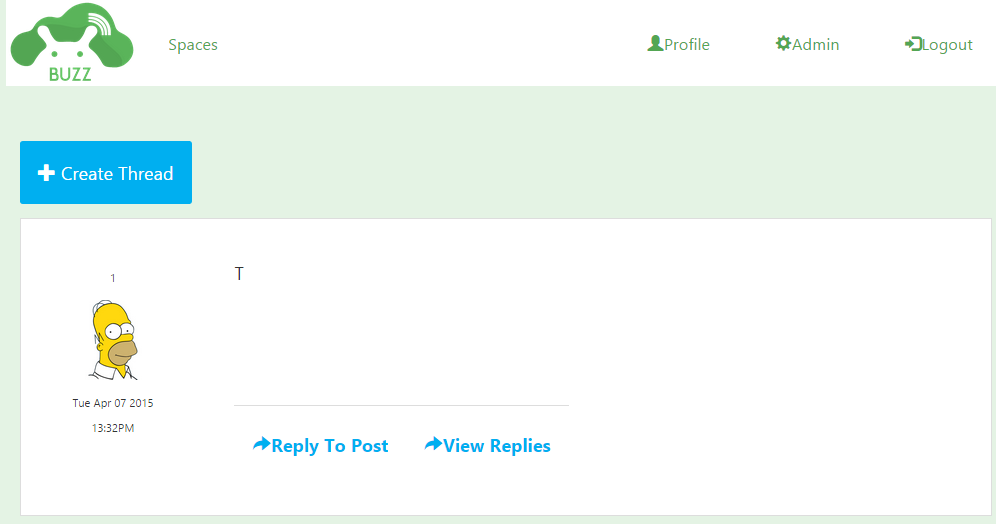
\includegraphics[width=0.85\textwidth]{No_appraisal}
    \caption{There are no appraisal icons that enables the user to "upvote" posts}
\end{figure}	
	\end{itemize}
\item assignAppraisalToPost:
	\begin{itemize}
		\item\textbf{Objective: } Allows the user to assign an appraisal to a post (i.e. rate a post).
		\item\textbf{Pre-conditions: }  Have a space where posts can be displayed.
		\item\textbf{Post-conditions: }The ranking/status of both the post and the user who posted the post will change.
		\item\textbf{Testing: } The pre-condition is not met as  the Buzz space does not function properly. This function was not implemented which means no post-conditions were met.
	\end{itemize}
\end{enumerate}
\end{enumerate}

\subsubsection{Non-functional Testing} 

\begin{enumerate}
\item Maintainability:

The Buzz(B) system is maintainable in the following aspects:

\begin{itemize}
\item Understandable by future developers:

Every subsystem or 'module' of the system is implemented as a seperate functioning module.
Standalone modules are then plugged into the system.
New developers can change modules independantly.
\item Technologies used is current and expected to be available for a long time:

Node.js makes up the core of the buzz system. It is a widely used open-source platform released in Q1 of 2009. Popularity has grown tremendously and is not expected to stop growing in the near future. 

MongoDB is used as a database structure of the Buzz system and is highly compatible with Node.js. Also released in 2009 and is now the fourth most popular type of database management system.  MongoDB is expected to grow even more in the coming years which makes it   a good choice for the Buzz system in terms of maintainability.

\item The system is easily updated

New functionality can be added by adding modules to the system.
Functionality can be changed by changing independat modules without having to rebuild the whole system.
\end{itemize}
\item Scalability

The Buzz(B) system is partially scalable in the following aspects:

\begin{itemize}
\item Able to host buzz spaces for all Computer Science modules:

The Buzz(B) system failed this scalability test. It does not support functionality of adding a new buzz space thus cannot host buzz spaces fot all CS modules.

\item University-wide, servicing in the order of 50 000 students:

The Buzz(B) system failed this scalability test. It does not support functionality of adding a new user or student. Thus one default user exists as apposed to 50 000.
\end{itemize}
\newpage
\item Auditability:

\textbf{Description}

The system needs to log all requests and all responses for all user services provided
by the system.

\textbf{Test Results}

The figure below shows that the Buzz Space system is partially auditable, only the requests for the user serves of the system are logged. The logged request only contains:
\begin{itemize}
\item User serves requested.
\item Request object stringified as JSON
\end{itemize}

There are no log responses that are provided by the system, and the serves required to extract information from the audit logs is also not available not provided.

\begin{figure}[h]
  \centering
    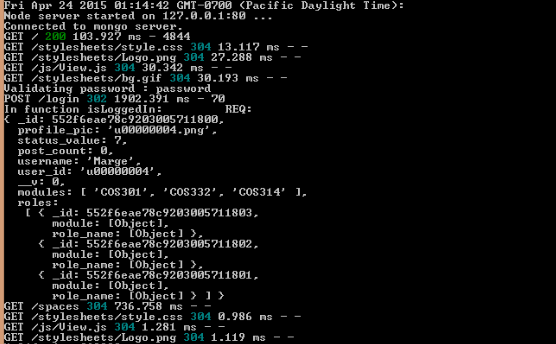
\includegraphics[width=0.85\textwidth]{BuzzBAuditability}
    \caption{Buzz Space B Auditability Test}
\end{figure}

\newpage
\item Testability:

\textbf{Description}

A system needs testabl through:
\begin{itemize}
\item Unit testing components in isolation
\item Integration tests where the components are integrated to the actual environment
\end{itemize}

\textbf{Test Results}
   
The Buzz system is divided into manageable components (modules) for each use case. Breaking the system into these components makes make the system testable through unit testing using mock objects. The Buzz system is a modular system, the system components are pluggable and makes automated integration testing simple as the component is integrated in the entire system.    
\item Performance requirements:

Requirements for the Buzz system were for non-reporting operations to preferably not last longer than 0.2 seconds and for report queries to be processed in no more than 5 seconds.
To test this we used Firebug, an open source web browser extension of Firefox used for webpage monitoring. (Version used: Firebug 2.0.7).
The Buzz system met these requirement:
\begin{itemize}
\item Non-reporting operations such as returning to a previous page (i.e. operations that relied on cached copies of a webpage) completed relatively close to the target time limit (e.g. returning to the main Buzz Spaces page after viewing the user’s profile took only 0.286 seconds, very close to the target time of 0.2 seconds).

\begin{figure}[h!]
  \centering
    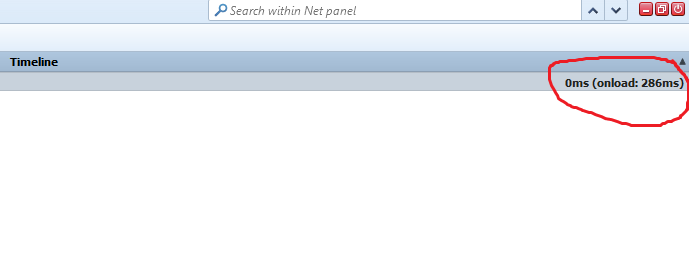
\includegraphics[width=0.85\textwidth]{Non-reporting_operationB}
    \caption{Non-reporting operation test}
\end{figure}

\item Report query operations (i.e. which had to communicate and receive some information from the system’s database) also completed within their desired time limit of 5 seconds (e.g. accessing the test module “TEST443”’s discussion space took only 1.24 seconds). Even some of the report query operations which took comparatively long to complete stayed within the 5 second limit (e.g. accessing module “COS332” took 4,81 seconds and accessing the Admin tab took 4,96 seconds).

\begin{figure}[h!]
  \centering
    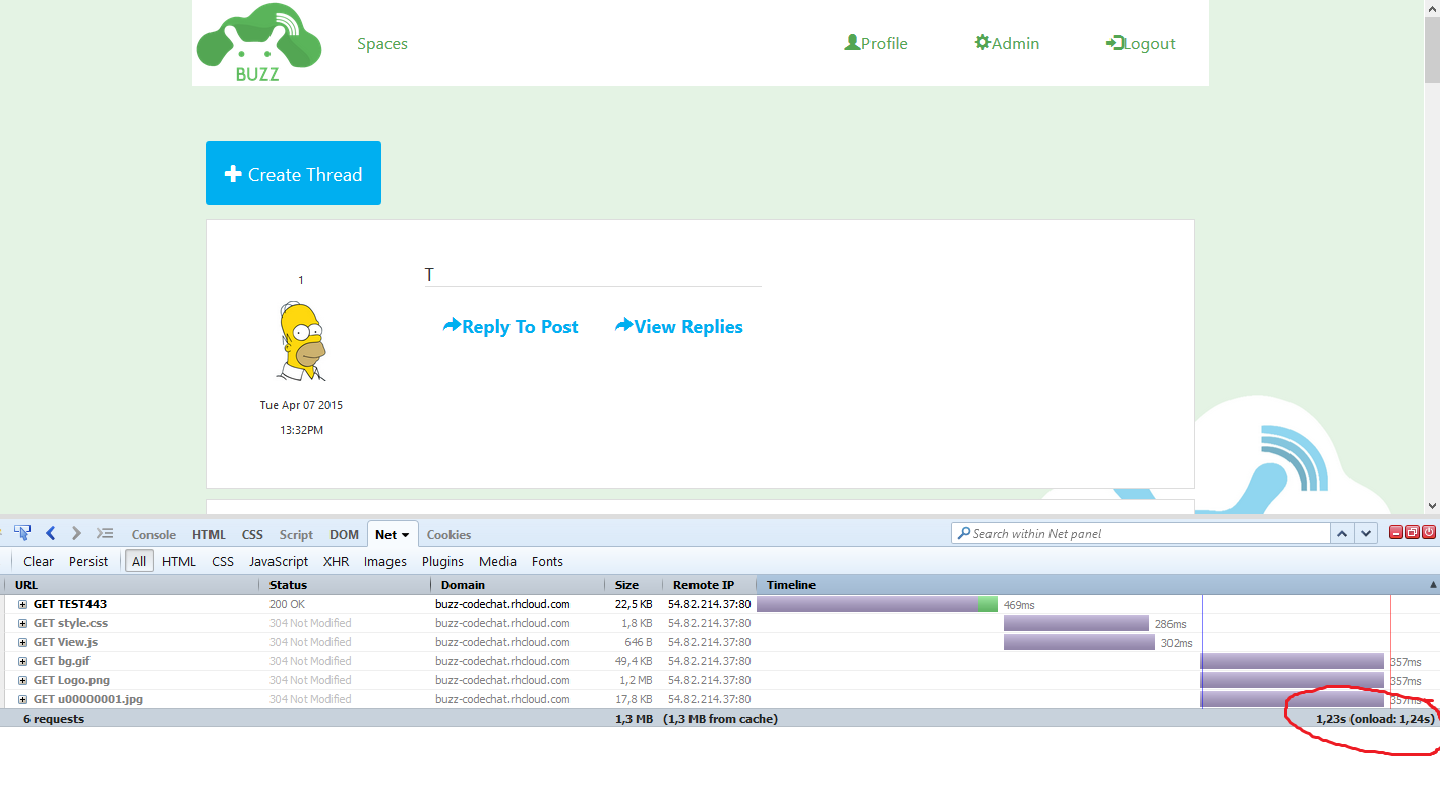
\includegraphics[width=0.85\textwidth]{Reporting_operationB}
    \caption{Reporting operation test}
\end{figure}

\end{itemize}	

\item Reliability and availability:

\begin{itemize}
	\item textbf{Availability: }
	The Buzz system can be accessed at the following URL (http://buzz-codechat.rhcloud.com/) at any time of day on any of the widely used 	web browsers (Google Chrome, Mozilla Firefox, Microsoft Internet Explorer, Safari and Opera). The Buzz system even functions and displays 	correctly on the web browsers of mobile devices to ensure maximum availability.
	\item textbf{Reliability: }
	The system performs various error checks to ensure that no user action could cause the Buzz system to fail/crash (e.g. returning error messages if the user tries to log on with incorrect information , Figure 3). Even in cases were the system’s functionaity was not fully implemented procedures are in place to rather warn the user of incomplete operations instead of blindly carrying out a harmful request (e.g. an error message is diplayed when a user tries to upload a new profile picture, Figure4). The reason why the Buzz system can still function (to an extent) even though much of its functional procedures are incomplete/missing is due to the modular fashion in which the system was created. Even if one module of the system fails it is appropriatley seperated from the other modules to prevent a complete system failure.

\begin{figure}[h!]
  \centering
    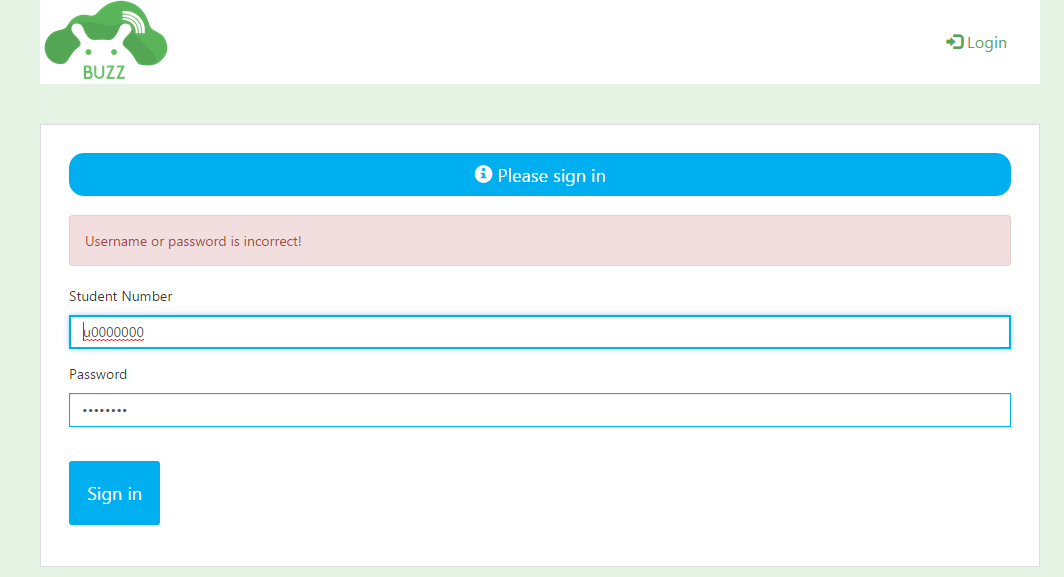
\includegraphics[width=0.85\textwidth]{ReliabilityB1}
    \caption{Login error}

\begin{figure}[h!]
  \centering
    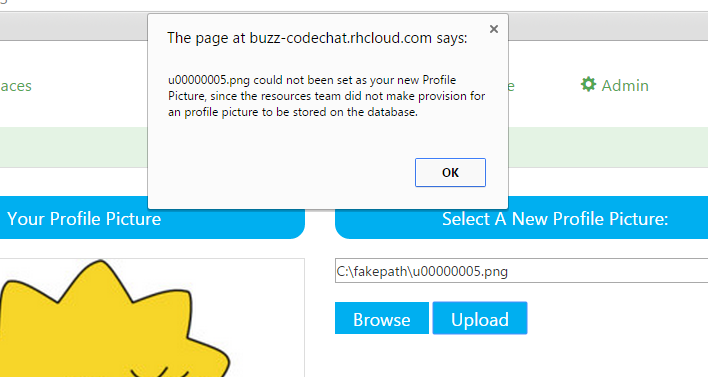
\includegraphics[width=0.85\textwidth]{ReliabilityB2}
    \caption{Error when uploading new profile picture}
\end{itemize}
	

\end{enumerate}

\end{document}
